\documentclass[11pt]{article}
\usepackage[utf8]{inputenc}
\usepackage{graphicx}
\usepackage{amsmath}
\usepackage{amsfonts}
\usepackage{hyperref}
\usepackage{listings}
\usepackage{courier}
\usepackage[letterpaper, portrait, margin=1in]{geometry}
\graphicspath{/home/black/CPS/euler}

\lstset{
	basicstyle=\footnotesize\ttfamily,
	frame=single,
	breaklines=true
}

\title{\vspace{-1.5cm}Project Eueler 107}
\author{Kevin Black}

\begin{document}

\maketitle

\section{Problem Statement}

The following undirected network consists of seven vertices and twelve edges with a total weight of 243.

\begin{center}
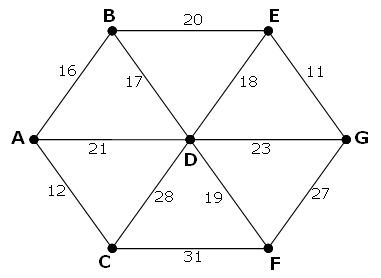
\includegraphics[scale=0.5]{/home/black/CPS/euler/p107_1.png}
\end{center}

The same network can be represented by the matrix below.

\begin{center}
\begin{tabular}{|c|c|c|c|c|c|c|c|}
\hline
 & A & B & C & D & E & F & G \\ \hline
A & - & 16	&12	&21	&-	&-	&- \\ \hline
B	&16	&-	&-	&17	&20	&-	&- \\ \hline
C	&12	&-	&-	&28	&-	&31	&- \\ \hline
D	&21	&17	&28	&-	&18	&19	&23 \\ \hline 
E	&-	&20	&-	&18	&-	&-	&11 \\ \hline
F	&-	&-	&31	&19	&-	&-	&27 \\ \hline
G	&-	&-	&-	&23	&11	&27	&- \\ \hline
\end{tabular}
\end{center}

However, it is possible to optimise the network by removing some edges and still ensure that all points on the network remain connected. The network which achieves the maximum saving is shown below. It has a weight of 93, representing a saving of 243 - 93 = 150 from the original network.

\begin{center}
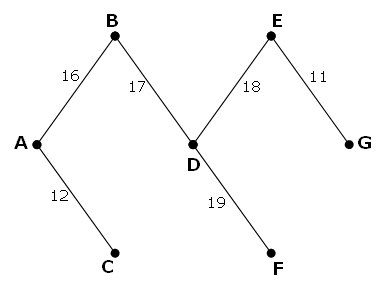
\includegraphics[scale=0.5]{/home/black/CPS/euler/p107_2.png}
\end{center}

Using network.txt (right click and 'Save Link/Target As...'), a 6K text file containing a network with forty vertices, and given in matrix form, find the maximum saving which can be achieved by removing redundant edges whilst ensuring that the network remains connected.


\section{Code}
\lstinputlisting[language=Python]{107.py}

\section{Rationale}
The first step is to regognize is that the resulting graph after achieving maximum saving is simply a minimum spanning tree for the original graph. You can then employ one of many MST finding algorithms to compute the weight of that tree, and subtract that from the total weight of the original graph to get the maximum saving.

The MST finding algorithm I chose is Prim's algorithm, which is a simple greedy algorithm that is an adaptation of Dijkstra's algorithm. It operates by maintaining a table $C$ of the vertices in the graph, where $C(v)$ is the cost of the cheapest path from $v$ to the partially built spanning tree. Each $C(v)$ is initialized to infinity, as there at first exists no path from each vertex to the tree, since the tree starts with no vertices. The algorithm then repeats the following steps:

\begin{enumerate}
	\item Choose the minimum value of $C(v)$, remove $v$ from $C$, and add $v$ to the tree.
	\item For each $w$ that is adjacent to $v$, update $C(w)$ if $vw < C(w)$.
\end{enumerate}

The algorithm terminates when $C$ is empty (all vertices are in the tree).

The time complexity of the algorithm is determined by the data structure used to store $C$. A simple list requires a linear search to find the minimum, making the total time complexity $O(V^2)$ where V is the number of vertices. I chose to instead use a min-heap, where finding the minimum takes constant time, but updating $C(w)$ (using a decrease-key operation) runs in $O(\log(n))$ time, making the total time complexity $O(E \log(V))$ where $E$ is the number of edges. However, the maximally efficient data structure for this algorithm is a Fibonacci heap, where the decrease-key operation runs in constant time, bringing the time complexity down to $O(E + V \log(V))$.

My code begins by reading and parsing the input file into a simple adjacency matrix called \verb!graph!, with a lack of a connection being represented as infinity. I then initialize my min-heap, with each key starting at infinity and the elements being the indices of the vertices. Finally, I compute the total weight of the graph from the adjacency matrix.

In the main loop, I repeat Prim's algorithm until my heap is empty, as described above. I first pop the minimum cost and its corresponding vertex off the heap, and subtract that cost from the total (since I am adding that vertex to the tree, and my eventual goal is to find the total weight minus the weight of the tree). The guard on that operation is just to prevent subtracting infinity from the total, which would only happen for the first vertex when the minimum is infinity. I then iterate through the entire heap to achieve step (2) of Prim's algorithm above. At first the code may seem different from step (2) described above since I am checking every vertex in $C$ rather than only those adjacent to $v$. However, if $v$ and $w$ are not adjacent, then \verb!graph[v][w]! is infinity, and the comparison \verb!graph[v][w] < wc! will never evaluate to true. Therefore, only adjacent vertices $w$ to $v$ will be updated, if the new cost $vw$ is less than what $C(w)$ was before. Updating the cost consists of simply changing the key in the heap, and then calling \verb!heapq._siftdown!, which performs the decrease-key operation to restore the heap invariants.

After the loop has terminated, \verb!total! will be the solution, since I have subtracted the cost of every edge in the minimum spanning tree.



\end{document}